\section{Upřesnění požadavků}
\change{rephrase}
Tvorba začala zjištěním požadavků. Udělal jsem Google formulář, který primárně zjišťoval informace o školním systému. Pomocí vedení školy byl pak rozeslán na spřátelené střední školy. 
\subsection{Výsledky průzkumu informačních systémů středních škol}
Na dotazník odpovědělo 13 škol z moravskoslezského kraje.

\begin{figure}[h]
    \centering
    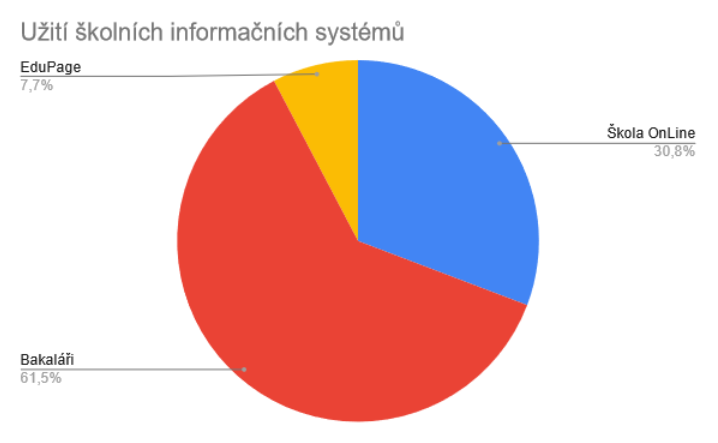
\includegraphics[width=0.5\linewidth]{Figures/vyuziti_skolnich_systemu.PNG}
    \caption{Využití školních informačních systémů}
    \label{fig:vyuziti-skolnich-systemu}
\end{figure}

Většina škol používá systém Bakaláři a na něj se bude zaměřovat import. Import bude možné udělat z tiskových sestav. Pro jiné školní systémy bude možno použít XML import, který je univerzální (podporuje i Bakaláře\footnote{Je však potřeba přístup k databázi Bakalářů a speciální program na vygenerování XML.}).


\newpage

\begin{figure}[t]
    \centering
    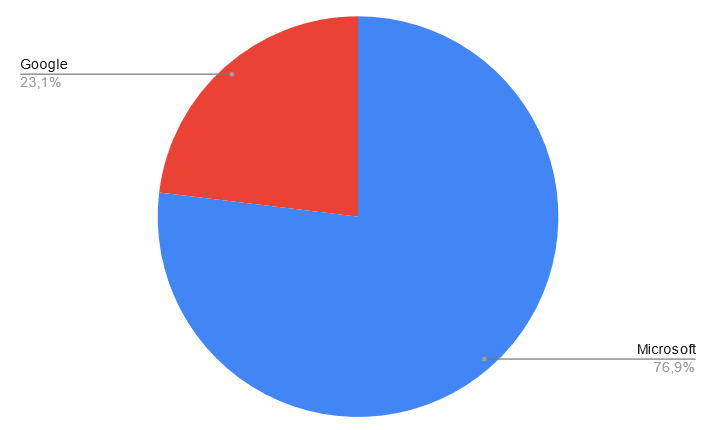
\includegraphics[width=0.5\linewidth]{Figures/poskytovatele_emailu.PNG}
    \caption{Poskytovatelé emailů}
    \label{fig:poskytovatele-emailu}
\end{figure}

Všechny dotazované školy mají emaily od Microsoftu nebo Googlu.
Přihlašování bude probíhat pomocí emailu. Uživatelé se budou moci přihlásit do portálu pomocí protokolu OAuth, který podporují oba provozovatelé. Výhodou tohoto způsobu přihlašování je, že naše aplikace neukládá hesla. Alternativně je možné ukládat heslo\footnote{Zahashované funkcí Bcrypt} do lokální databáze.

\section{Použité technologie}

Používáme framework \href{https://symfony.com/}{Symfony}. Symfony je open-source PHP framework, který je vydán pod MIT licencí.  Využívá návrhový vzor MVC a moderní PHP. Symfony je modulární a jednoduše rozšiřitelný pomocí existujících bundlů/componentů. To je jeden z hlavních důvodů, proč byl tento framework vybrán. Již spoustu problémů řeší za nás a zamezuje tím bezpečnostním a jiným chybám.

Používáme Symfony společně s Doctrine ORM, to nám poskytuje řadu výhod jako typesafe mapování, nezávislost na databázi\footnote{Doctrine ORM aktuálně podporuje PostgreSQL, MySQL, Oracle, SQL server a další\cite{doctrine-supported-dbs}}. S Doctrine používáme přístup code first, napíšeme standardní PHP třídu, kde pomocí atributů přidáme vlastnostem informace o jejich mapování. 
\unsure{Pridat example}
Za zmíňku stojí Symfony EasyAdmin, který dokáže vytvořit pro danou entitu CRUD stránku, která je jednoduše upravitelná.

Jako web server používáme FrankenPHP, moderní php server založený na serveru Caddy. FrankenPHP podporuje worker mode, který umožňuje znovu použití PHP interpretoru při dalším requestu.

Pro uchovávání dat používáme relační databázi PostgreSQL, ta podporuje  pokročilejší funkce jako transakce DDL, narozdíl od MySQL.  

Naše aplikace je nasazována pomocí dockeru. Pro každou školu máme zvlášť container s databázovým a webovým serverem. Jako reverse proxy používáme Traefic, který nám umožňuje jednoduchou správu instancí.



\section{Návrh databáze}

\improvement{Vložit schéma db: }



\section{Způsoby importu}
Při prvotním importu, kdy se načítají informace o studentech a úvazcích se rovnou vytváří entity. Entity se ale nepersistují hned a ukládají se do databáze až v ImportService.

Importy z XML a sestav splňují interface ImportDataProvider. Ten se skládá z getterů vracejících managery. Managery jsou objekty, co se starají o správu daných entit. ImportService potom příjme ImportDataProvider a postará se o jeho uložení. ImportService se dá doplnit o další postup ukládání typu ImportSaveStep, další postup závisí na formátu ze kterého se importuje.

\section{Import z tiskových sestav systému Bakaláři}
\improvement{proofread}
Tento typ importu slouží pro školy, které nemají přístup k databázi Bakalářů. 
Jedná se primárně o školy, které využívají cloud verzi Bakalářů. Využívají se tři sestavy, které jsou již předvytvořené\unsure{Doufám, že nejsou custom}. Bakaláři používají XFRX\footnote{Knihovna, která převádí Visual FoxPro reporty na elektronické sestavy různých formátů} ke generování samotných sestav. Tyto sestavy nejsou určeny ke zpětnému programatickému čtení dat.

Dostupné formáty sestav jsou TXT, CSV, XLS a HTML. U sestav formátu TXT chybí mezery jako separátor u sloupců, sestava předmětů ve formátu CSV by byla možná importovat, ale ostatní sestavy by nešly jednoduše zpracovat kvůli zdánlivě náhodnému počtu separátorů, podobný problém nastává i u XLS tam se však ještě vyskytuje problém se sloučenými poli.

Zvolil jsem, že budu importovat HTML sestavy. Celá tabulka je postavená na základě absolutního pozicování. Při parsování sestav seřadím jednotlivé divy podle absolutního pozicování. Tímto způsobem převádím každý řádek v tabulce na objekt.

Sestava úvazků však obsahuje řadu chyb. Když učitel zárověň učí více tříd najednou, objeví se ve sloupci třídy nevalidní zkratky tříd. Toto řeším vyhledáním třídy a skupiny v sestavě tříd na základě členů skupiny. 
Zkratky předmětu jsou správné, až na případ když se daný předmět dělí na teorii a cvičení,
kvůli tohoto je potřeba najít v sestavě předmětů správnou zkratku. Někdy se stane, že název předmětu není úplný a potom se vezme zkratka ze sestavy předmětů.

Nula ve sloupci týdně znamená, že daný učitel tento úvazek\unsure{co je uvazek} aktuálně neučí, to muže nastat při rotaci skupin nebo u teorií daného předmětu, které učitel neučí\improvement{rephrase}. 

\begin{figure}[h]
    \centering
    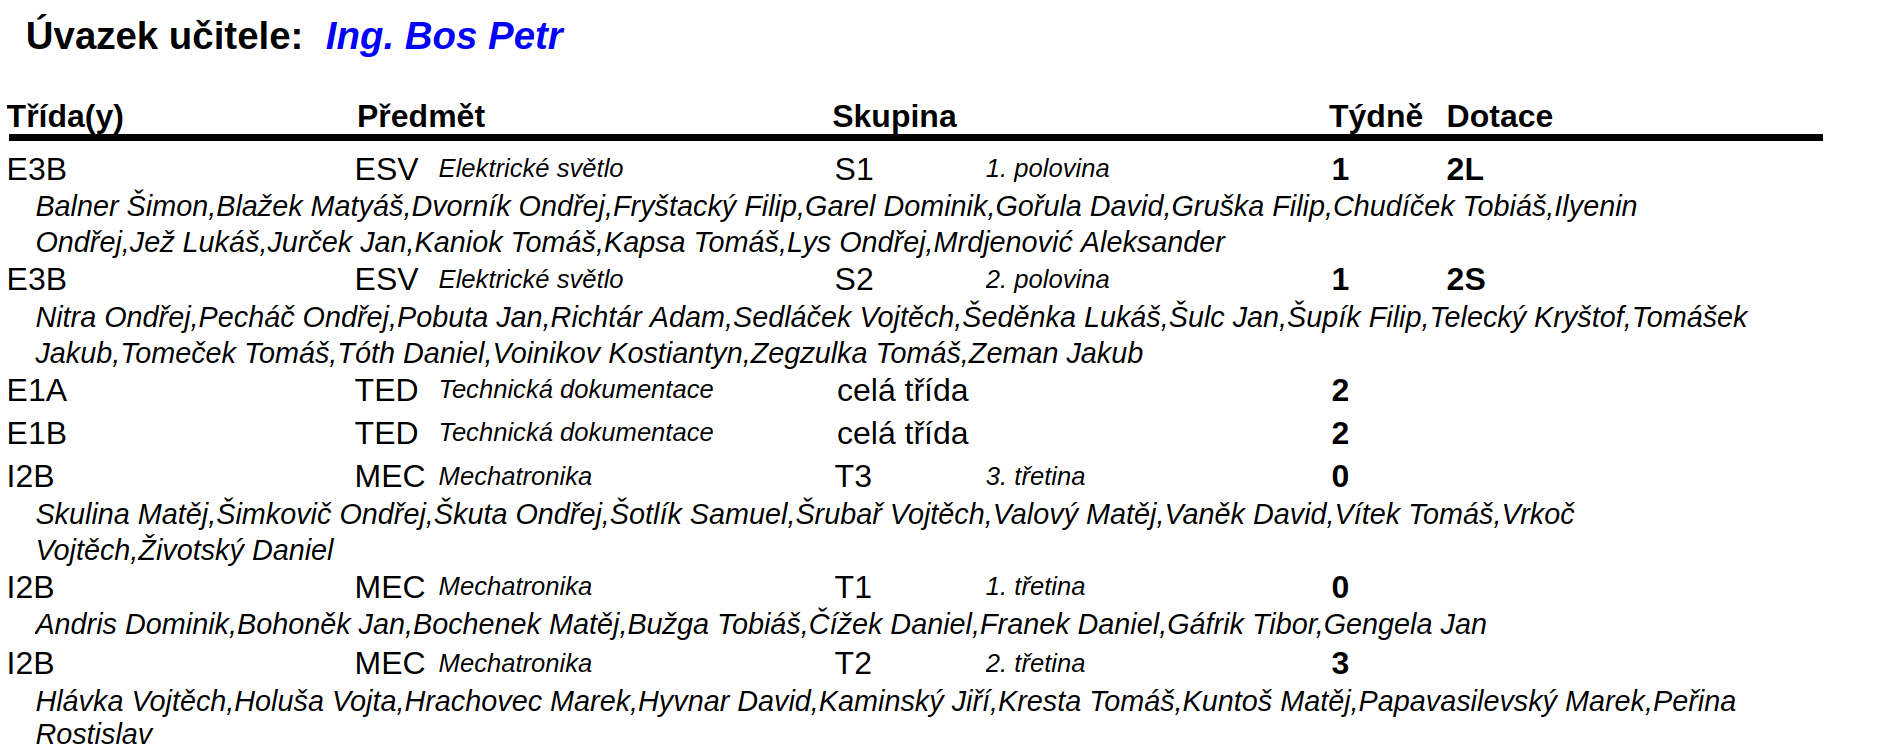
\includegraphics[width=1\linewidth]{Figures/uvazky-ucitelu-ukazka.png}
    \caption{Ukázka sestavy obsahující úvazky učitelů}
    \label{fig:uvazky-ucitelu-ukazka}
\end{figure}

\begin{figure}[H]
    \centering
    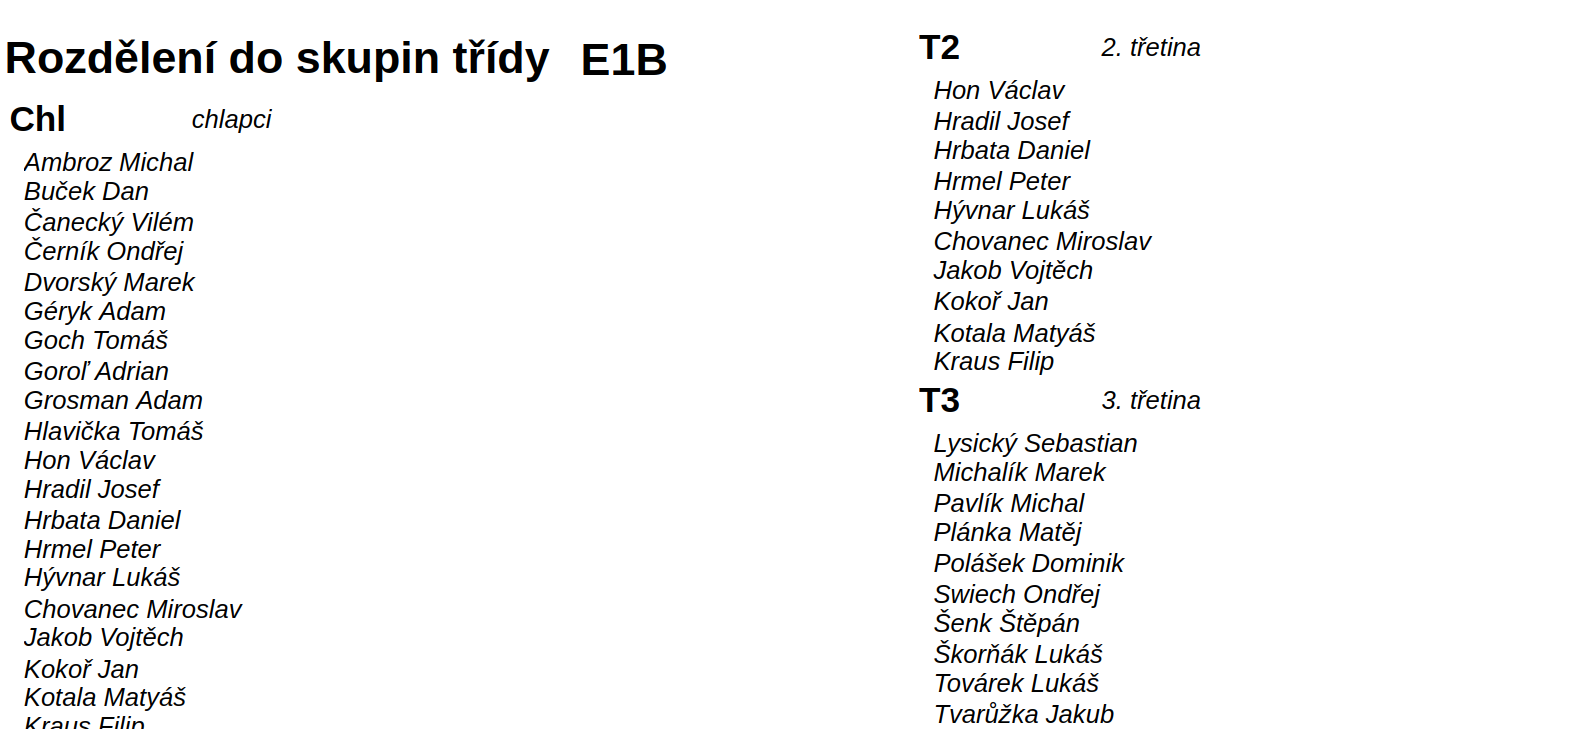
\includegraphics[width=1\linewidth]{Figures/skupiny-ukazka.png}
    \caption{Ukázka sestavy rozdělení studentů do tříd}
    \label{fig:ukazka-sestavy-tridy}

\end{figure}
\begin{figure}[H]

    \centering
    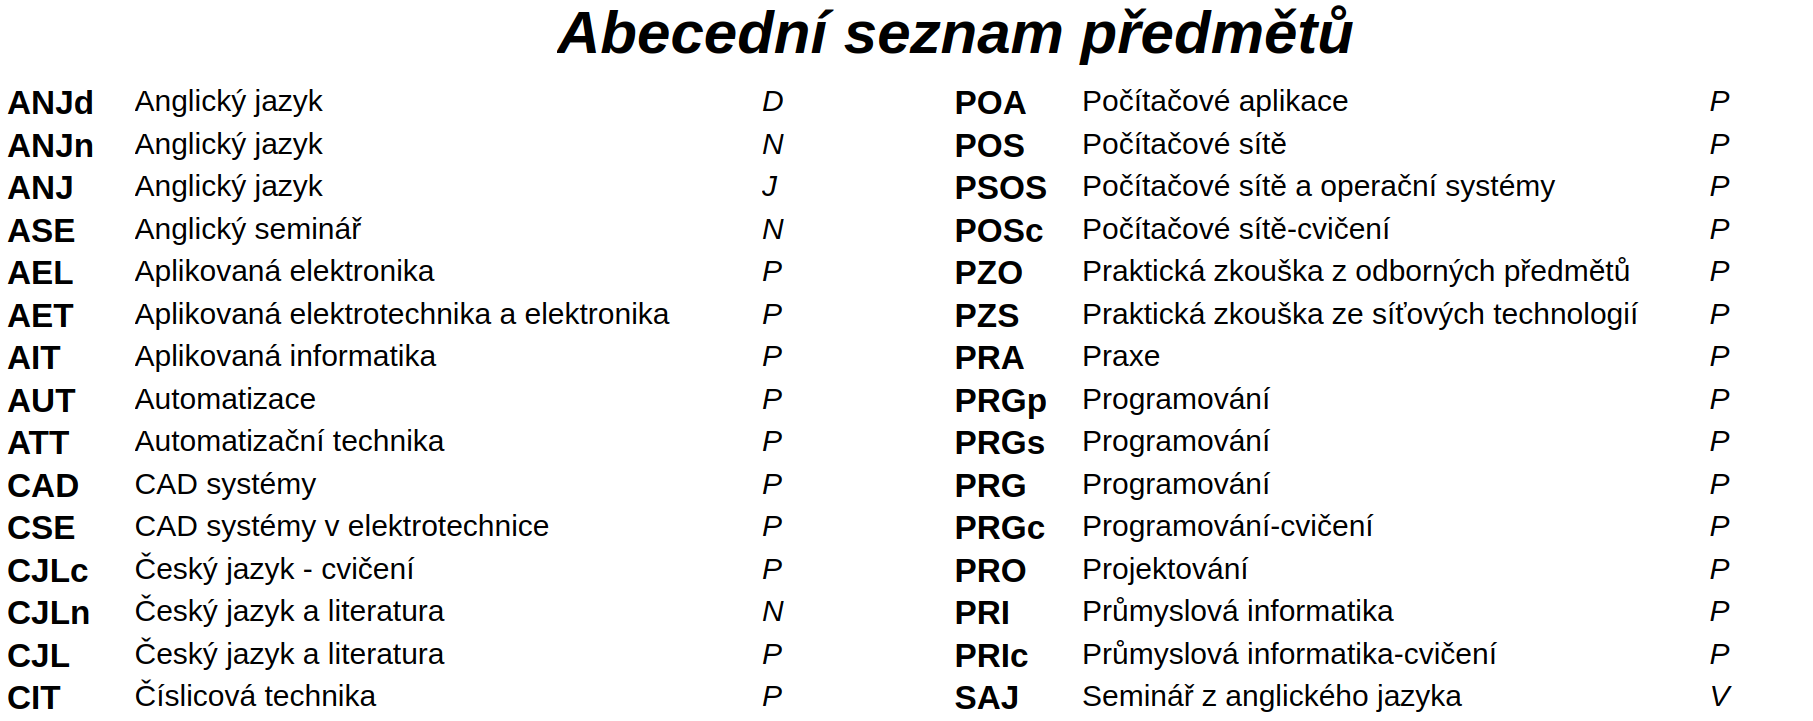
\includegraphics[width=1\linewidth]{Figures/predmety-ukazka.png}
    \caption{Ukázka sestavy předměty}
    \label{fig:ukazka-sestavy-predmety}
    
\end{figure}
\begin{figure}[H]
\begin{lstlisting}[language=HTML,caption={Zkrácené zdrojové HTML sestavy}]
<div class="page" style="width:794;height:1123;"><a name="XFRXPAGE_1">
 ...
 <div class="font7" style="top:30px;left:129px;height:19px;width:230px;...">Ing. Bos Petr</div>
 <div class="font6" style="top:30px;left:4px;height:20px;width:128px;...">Úvazek učitele:</div>
 <div class="base" style="border-width:0px;border-top-width:2px;top:80px;left:-3px;height:1px;width:756px;border-style:solid;border-color:RGB(0,0,0);background-color:RGB(0,0,0);"></div>
 <div class="font2" style="top:103px;left:8px;height:30px;width:745px;...">Balner Šimon,Blažek Matyáš,Dvorník Ondřej,Fryštacký Filip,Garel Dominik,Gořula David,Gruška Filip,Chudíček Tobiáš,Ilyenin</div>
 ...
</div>
\end{lstlisting}
\end{figure}


\section{Import z XML}
Import z XML je nezávislý na školním systému. Je však potřeba mít externí program, který XML vytvoří dle daného schématu (schéma je v souboru\improvement{nazev souboru}). Struktura je použitá z předchozí verze (více v \ref{uvod:predchozi-verze}), kořenový prvek se jmenuje BakalariImport z historických důvodu. Emaily jsou v dobrovolné a pokud budou u některých studentů/učitelů chybět vygenerují se v dalším kroku importu.

Na import XML se používá PHP extension SimpleXML. Je to jednoduchý způsob parsování. Jediná nevýhoda je, že SimpleXML načte celý soubor XML do paměti. XML soubory škol jsou však malé a i kdyby měla škola počet žáků v řádech tisíců, SimpleXML by dostačovalo. 



\definecolor{gray}{rgb}{0.4,0.4,0.4}
\definecolor{darkblue}{rgb}{0.0,0.0,0.6}
\definecolor{cyan}{rgb}{0.0,0.6,0.6}


\lstdefinelanguage{XML}
{
  morestring=[b]",
  morestring=[s]{>}{<},
  morecomment=[s]{<?}{?>},
  stringstyle=\color{black},
  identifierstyle=\color{darkblue},
  keywordstyle=\color{cyan},
  morekeywords={xmlns,version,type}% list your attributes here
}
\begin{lstlisting}[language=XML,basicstyle=\small,caption={Ukázka struktury XML}]
<?xml version="1.0" encoding="utf-8"?>
<BakalariImport>
    <SkolniRok>2022/23</SkolniRok>
    <Predmety><Predmet><Zkratka>PRG</Zkratka><Nazev>Programování</Nazev></Predmet>
    </Predmety>
    <Studenti>
        <Student>
            <Jmeno>Marek</Jmeno>
            <Prijmeni>Konrád</Prijmeni>
            <!-- Email není povinný -->
            <Email>m.konrad.st@spseiostrava.cz</Email>
            <Trida>I4C</Trida>
            <Skupiny><Skupina>S1</Skupina></Skupiny>
        </Student>
    </Studenti>
    <Ucitele>
        <Ucitel>
            <Jmeno>Vlasta</Jmeno>
            <Prijmeni>Kubinová</Prijmeni>
            <Titul>Mgr.</Titul>
            <!-- Email není povinný -->
            <Email>v.kubinová@spseiostrava.cz</Email>
            <Zkratka>NOW</Zkratka>
            <Predmety>
                <Predmet>
                    <Zkratka>PRG</Zkratka>
                    <Tridy>
                        <Trida>
                            <Zkratka>I4C</Zkratka>
                            <Skupina>S1</Skupina>
                        </Trida>
                    </Tridy>
                </Predmet>
            </Predmety>
        </Ucitel>       
    </Ucitele>
</BakalariImport>
\end{lstlisting}


\section{Databáze a mapování importu}

Importy závisí na školní rok. Když vytvoříte školní rok nemáte žádná data. Každé hodnocení probíhá od začátku školního roku až po moment nejnovějšího importu.

Ukládání importu do databáze probíhá pomocí ORM. Máme vytvořené třídy a Doctrine už je mapuje na tabulky v relační databázi. Doctrine dokáže mapovat celou řadu OOP konceptů jako dědičnost a kompozici.

Uživatele máme řešené dědičností tak, že třídy \codename{Student} a \codename{Teacher} dědí z abstraktní třídy \codename{ImportedPerson} a ta dědí ze třídy \codename{User}. Takto uspořádaná hierarchie tříd má řadu výhod jako možnost dotazovat všechny importované osoby najednou. \improvement{toto se využívá v ... ref} Nevýhoda takovéhoto mapování je zvýšená komplexita pro ORM a potencionální degradace výkonu z databázové strany.

Doctrine je ORM se silnou abstrakcí, což značně komplikuje samotné ukládání. Není totiž podporovaná operace (v databázi PostgreSQL realizovanou pomocí jednoho dotazu INSERT INTO ... ON CONFLICT DO UPDATE). Je sice možné užít nativní SQL, ale tím bychom přišli o výhody ORM.
Nevýhodou je pomalejší ukládání, to se děje kvůli tomu, že Doctrine se snaží vytvořit graf daných entit, Doctrine interně používá identity map na entity takže je vyšší spotřeba RAM.



\section{Inkrementální import}

Zdroje importů nemusí poskytovat data o celém školním roce, v případě importu ze sestav se jedná o úvazky, kde se střídají skupiny u učitele (na naší škole např. mechatronika).
 Nebo se během školního roku něco nečekaně změní.

Proto umožňujeme inkrementální import, importuje se jen to nové a staré importy nechává nedotčené. Doporučuji dělat import před každým testovacím obdobím. Data ze starých importů není třeba odstraňovat (i staré úvazky, které už nemusí být platné lze hodnotit). 

Entity spravované importem implementují interface \codename{ImportedEntity}.

\begin{lstlisting}[language=PHP, caption={Zdrojový kód \codename{ImportedEntity}}]
    interface ImportedEntity
    {
        public function getId(): mixed;
    
        public function getImportHash(): ?string;   

        public function loadImportHash(): string;   
        public function updateFromSelf(ImportedEntity $old): static;
    }
\end{lstlisting}

V Doctrine se dělají hromadné operace po $N$ operacích. $N$ se dá zvolit experimentem.
Po každých $N$ operacích se pak zavolají metody \codename{EntityManager.flush()} a \codename{EntityManager.clear()}. Dělá se to po inkrementech, aby \codename{UnitOfWork} byl schopen udělat možné optimalizace a aby se zamezilo zbytečnému procházení grafu entit. Operace clear pak vyčistí graf, to je důležité aby nedošlo k úniku paměti.

\codename{ImportedEntity} má metody loadImportHash ta se používá ke vytvoření import hashe. Import hash se skládá z atributů, které unikátně identifikují danou entitu. Pro import nelze spoléhat na dané atributy, protože uživatel je může prostřednictvím administrace upravit. To by znamenalo, že při dalším importu bude stejná instance entity znovu vytvořena\footnote{Kdyby chtěl uživatel, aby byla při dalším importu vytvořena nová instance entity, může vymazat hodnotu import hashe.}.
Import hash je využíván třídou \codename{ImportedEntityUpsertProcessor}. Ten se stará o upsert importovaných entit.
\codename{ImportedEntityUpsertProcessor} načte při upsertu všechny instance ukládané entity. Potom vytvoří \codename{entityMap}, což je mapa import hashů na id.  

\section{O korcích importu}





\section{Generování emailů z uživatelských dat}

\section{Deduplikace generovaných emailů}

